\documentclass[11pt]{article}
\usepackage[utf8]{inputenc}
\usepackage{amsmath}
\usepackage{amssymb}
\usepackage{geometry}
\usepackage{booktabs}
\usepackage{fancyhdr}
\usepackage{graphicx}
\usepackage{float}
\usepackage{listings}
\usepackage{xcolor}
\usepackage{titlesec}
\usepackage{adjustbox}
\usepackage{hyperref}

\titleformat{\section}{\normalfont\large\bfseries}{\thesection}{1em}{}
\titleformat{\subsection}{\normalfont\normalsize\bfseries}{\thesubsection}{1em}{}

\definecolor{codegreen}{rgb}{0,0.6,0}
\definecolor{codegray}{rgb}{0.5,0.5,0.5}
\definecolor{codepurple}{rgb}{0.58,0,0.82}
\definecolor{backcolour}{rgb}{0.95,0.95,0.92}

\lstdefinestyle{mystyle}{
  backgroundcolor=\color{backcolour},
  commentstyle=\color{codegreen},
  keywordstyle=\color{magenta},
  numberstyle=\tiny\color{codegray},
  stringstyle=\color{codepurple},
  basicstyle=\ttfamily\footnotesize,
  breakatwhitespace=false,
  breaklines=true,
  captionpos=b,
  keepspaces=true,
  numbers=left,
  numbersep=5pt,
  showspaces=false,
  showstringspaces=false,
  showtabs=false,
  tabsize=2
}
\lstset{style=mystyle}

\geometry{a4paper, margin=1in}
\setlength{\parindent}{0pt}
\setlength{\parskip}{0.5em}
\setlength{\headheight}{15pt}

\pagestyle{fancy}
\fancyhf{}
\lhead{Spring 2026 Intro to Deep Learning}
\rhead{Final Project --- Type-A}
\rfoot{Page \thepage}

\begin{document}

% ── Title block ────────────────────────────────────────────────────────────────
\begin{center}
  {\Large \textbf{Evaluating Dropout and Batch Normalization on LeNet-5}} \\
  \vspace{0.2cm}
  {\large Final Project --- Type-A, Topic 3} \\
  \vspace{0.2cm}
  \textbf{Course:} Spring 2026 Introduction to Deep Learning \\
  \textbf{Name:} Karim Smires \\
  \textbf{Due Date:} May 13, 2026
\end{center}
\hrule
\vspace{0.5cm}

% ── Abstract ──────────────────────────────────────────────────────────────────
\section*{Abstract}
This project investigates the effect of two common regularization techniques---Dropout
applied to fully-connected (FC) layers and Batch Normalization (BN) applied to
convolutional layers---on a LeNet-5 network trained to classify handwritten digits
from the MNIST dataset. Four configurations are evaluated in a $2\times 2$ factorial
design (Dropout on/off $\times$ BN on/off). Each configuration is trained with five
independent random seeds to report statistically reliable mean and standard deviation
of test accuracy. Results show that Dropout provides the larger accuracy gain
($\approx$0.18\%), that BN provides a smaller but consistent benefit, and that combining
both techniques yields the highest test accuracy of $99.14\% \pm 0.05\%$ while also
achieving the lowest train-to-test generalization gap.

% ── Introduction ──────────────────────────────────────────────────────────────
\section{Introduction}
Overfitting is a central challenge in training deep neural networks: a model may memorize
the training set and fail to generalize to unseen data. Two widely adopted countermeasures
are Dropout \cite{srivastava2014dropout} and Batch Normalization \cite{ioffe2015batch}.
Dropout randomly deactivates neurons during training, acting as an ensemble of many
sub-networks. Batch Normalization normalizes the activations within each mini-batch,
reducing internal covariate shift and providing a mild regularization effect.

While both techniques are well-studied individually, their interaction is less obvious: BN
can reduce the need for Dropout in some settings, and Dropout can interfere with BN's
running statistics if applied incorrectly. This project uses LeNet-5 on MNIST as a
controlled testbed to answer the following question: \textit{which combination of FC Dropout
and convolutional BN produces the best generalization performance?}

% ── Related Work ──────────────────────────────────────────────────────────────
\section{Related Work}
\textbf{LeNet-5} \cite{lecun1998gradient} is a pioneering convolutional neural network
introduced by LeCun et al.\ for handwritten digit recognition. It consists of two
convolutional layers followed by three fully-connected layers and established the template
for modern CNNs.

\textbf{Dropout} \cite{srivastava2014dropout} was proposed by Srivastava et al.\ as a
simple regularization method: during each training step, each neuron is independently
zeroed with probability $p$, preventing co-adaptation of features.

\textbf{Batch Normalization} \cite{ioffe2015batch} was introduced by Ioffe and Szegedy to
address internal covariate shift. By normalizing layer inputs over the mini-batch,
it allows higher learning rates, reduces sensitivity to initialization, and acts as
a regularizer. It has been shown to accelerate convergence, especially in convolutional
networks.

% ── Data Description ──────────────────────────────────────────────────────────
\section{Data Description}
The MNIST dataset \cite{lecun1998gradient} consists of $70{,}000$ grayscale images of
handwritten digits (0--9), each of size $28\times28$ pixels.

\begin{itemize}
  \item \textbf{Training set:} 60,000 images
  \item \textbf{Test set:} 10,000 images
  \item \textbf{Classes:} 10 (digits 0--9), balanced across splits
\end{itemize}

Images are normalized to zero mean and unit variance using the channel-wise statistics
$\mu = 0.1307$, $\sigma = 0.3081$ prior to all experiments. No data augmentation is applied.

% ── Method Description ────────────────────────────────────────────────────────
\section{Method Description}

\subsection{Dropout}
At each training iteration, every neuron in a targeted layer is independently set to zero
with probability $p$ (here $p=0.5$). During inference the Dropout layer is disabled and
activations are used as-is; PyTorch scales activations by $1/(1-p)$ during training
so no additional rescaling is needed at test time. Dropout is applied after both
hidden FC layers (FC1 and FC2) but not after the output layer.

\subsection{Batch Normalization}
For a mini-batch of activations $\{x_i\}_{i=1}^{N}$, BN computes:
\[
  \hat{x}_i = \frac{x_i - \mu_\mathcal{B}}{\sqrt{\sigma^2_\mathcal{B} + \epsilon}},
  \qquad
  y_i = \gamma \hat{x}_i + \beta
\]
where $\mu_\mathcal{B}$ and $\sigma^2_\mathcal{B}$ are the mini-batch mean and variance,
and $\gamma$, $\beta$ are learned scale and shift parameters. BN is inserted after each
convolutional layer and before the ReLU activation, following the convention of
\cite{ioffe2015batch}.

% ── Model Description ─────────────────────────────────────────────────────────
\section{Model Description}

The base architecture is a modern variant of LeNet-5 adapted for $28\times28$ MNIST input:

\begin{table}[H]
  \centering
  \begin{tabular}{llll}
    \toprule
    \textbf{Layer} & \textbf{Operation} & \textbf{Output Shape} & \textbf{Notes} \\
    \midrule
    Input  & ---                         & $1\times28\times28$ & \\
    Conv1  & Conv2d($1{\to}6$, $5\times5$) & $6\times24\times24$ & [BN] $\to$ ReLU $\to$ MaxPool \\
    Pool1  & MaxPool2d($2\times2$)         & $6\times12\times12$ & \\
    Conv2  & Conv2d($6{\to}16$, $5\times5$)& $16\times8\times8$  & [BN] $\to$ ReLU $\to$ MaxPool \\
    Pool2  & MaxPool2d($2\times2$)         & $16\times4\times4$  & \\
    Flatten& ---                         & $256$               & \\
    FC1    & Linear($256{\to}120$)        & $120$               & ReLU $\to$ [Dropout] \\
    FC2    & Linear($120{\to}84$)         & $84$                & ReLU $\to$ [Dropout] \\
    FC3    & Linear($84{\to}10$)          & $10$                & Output logits \\
    \bottomrule
  \end{tabular}
  \caption{LeNet-5 architecture. Bracketed components are conditionally present.}
\end{table}

The four experimental configurations are:

\begin{enumerate}
  \item \textbf{Config 1 --- FC-Dropout + CONV-BN:} Dropout in FC1/FC2; BN in Conv1/Conv2.
  \item \textbf{Config 2 --- FC-Dropout + CONV-noBN:} Dropout in FC1/FC2; no BN.
  \item \textbf{Config 3 --- FC-noDropout + CONV-BN:} No Dropout; BN in Conv1/Conv2.
  \item \textbf{Config 4 --- FC-noDropout + CONV-noBN:} Baseline; no Dropout, no BN.
\end{enumerate}

% ── Experimental Procedure and Results ────────────────────────────────────────
\section{Experimental Procedure and Results}

\subsection{Experimental Setup}
All experiments are implemented in PyTorch 2.11.0 and executed on an NVIDIA RTX 5070 GPU.

\begin{table}[H]
  \centering
  \begin{tabular}{ll}
    \toprule
    \textbf{Hyperparameter} & \textbf{Value} \\
    \midrule
    Optimizer    & Adam \\
    Learning rate & 0.001 \\
    Batch size   & 128 \\
    Epochs       & 20 \\
    Dropout rate & 0.5 \\
    Random seeds & 5 (seeds 0--4) \\
    \bottomrule
  \end{tabular}
  \caption{Hyperparameters used across all configurations.}
\end{table}

Each configuration is trained five times with different random seeds. Final test accuracy
(epoch 20) and best test accuracy (highest over all epochs) are recorded per seed, and
mean $\pm$ standard deviation are reported.

\subsection{Results}

\begin{table}[H]
  \centering
  \adjustbox{max width=\textwidth}{%
    \begin{tabular}{lcccc}
      \toprule
      \textbf{Configuration} & \textbf{Final Test Acc} & \textbf{Best Test Acc} & \textbf{Train Acc (ep.20)} & \textbf{Time} \\
      \midrule
      Config 1: FC-Dropout + CONV-BN    & $\mathbf{99.14\% \pm 0.05\%}$ & $\mathbf{99.20\% \pm 0.03\%}$ & $98.94\%$ & 98.7 s \\
      Config 2: FC-Dropout + CONV-noBN  & $99.13\% \pm 0.05\%$          & $99.19\% \pm 0.05\%$          & $98.89\%$ & 93.8 s \\
      Config 3: FC-noDropout + CONV-BN  & $98.96\% \pm 0.12\%$          & $99.14\% \pm 0.06\%$          & $99.76\%$ & 101.3 s \\
      Config 4: FC-noDropout + CONV-noBN& $98.94\% \pm 0.08\%$          & $99.05\% \pm 0.04\%$          & $99.72\%$ & 103.1 s \\
      \bottomrule
  \end{tabular}}
  \caption{Test accuracy (mean $\pm$ std over 5 seeds) and final epoch training accuracy.
  Time is total wall-clock time for all 5 seeds.}
\end{table}

\begin{figure}[H]
  \centering
  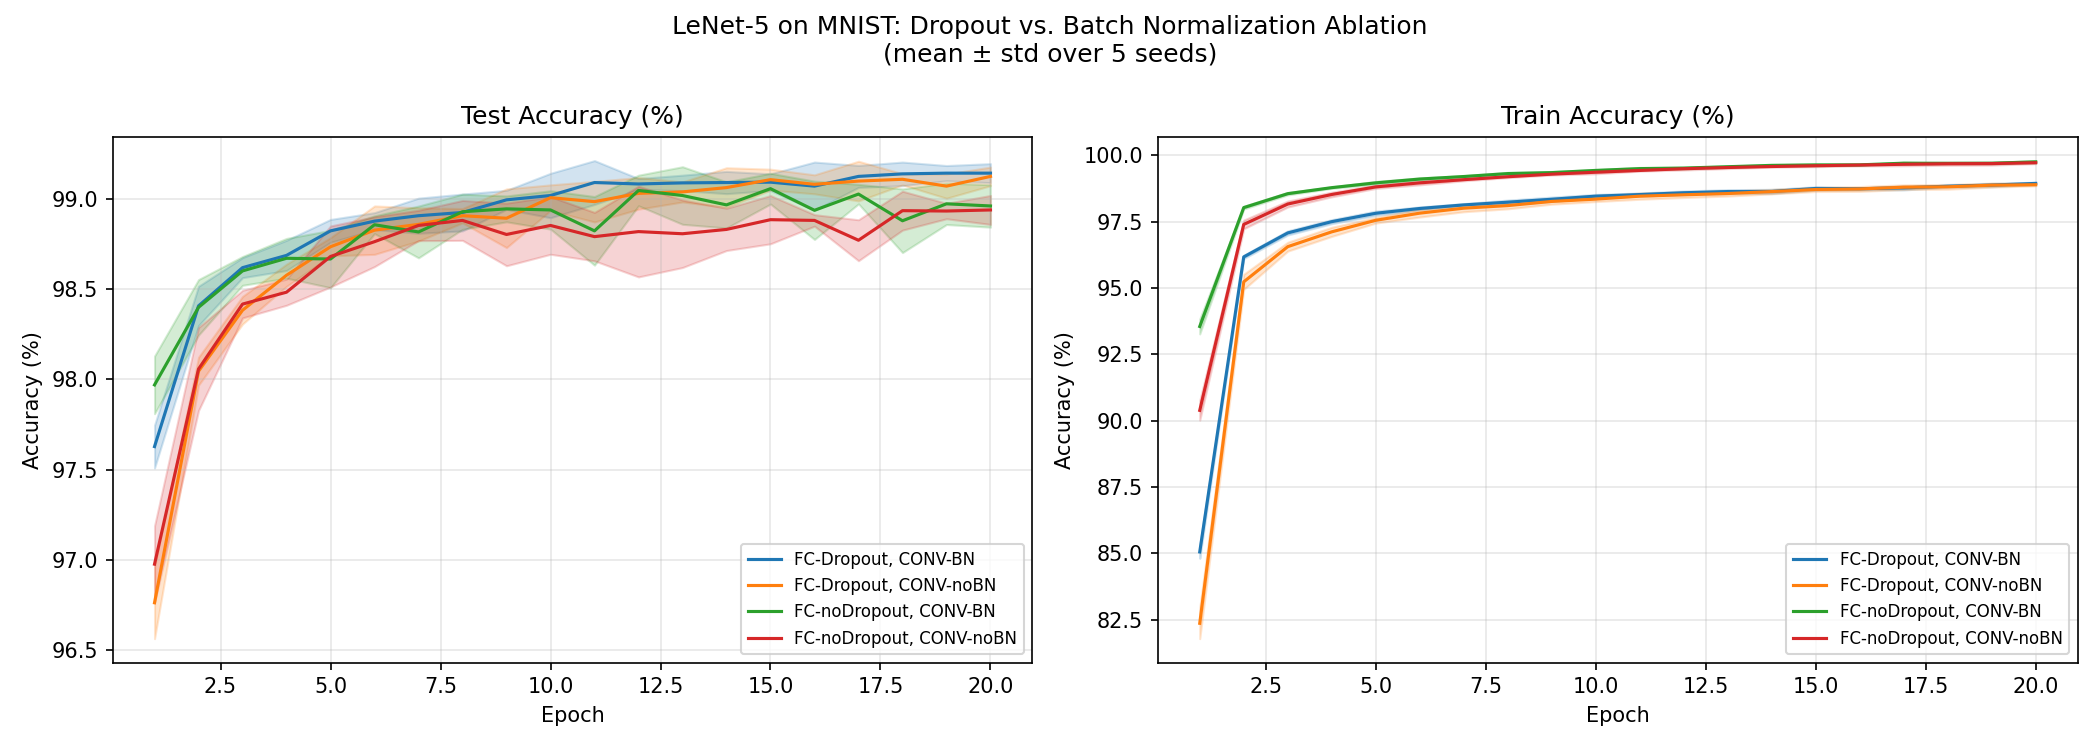
\includegraphics[width=\textwidth]{../results.png}
  \caption{Test accuracy (left) and training accuracy (right) over 20 epochs.
  Shaded bands show $\pm 1$ standard deviation across 5 seeds.}
  \label{fig:results}
\end{figure}

\subsection{Analysis}

\textbf{Config 1 (FC-Dropout + CONV-BN) achieves the highest performance} in both final
and best test accuracy, confirming that the combination of both regularization techniques
is optimal.

\textbf{Dropout has a larger impact than BN.} Comparing configurations with and without
Dropout (holding BN constant), Dropout contributes a $\approx$0.18\% gain in test
accuracy. The corresponding gain from BN alone (holding Dropout constant) is much smaller,
at only $\approx$0.02\%.

\textbf{Dropout significantly reduces overfitting.} Without Dropout (Configs 3 and 4),
training accuracy reaches $\approx$99.7--99.8\% while test accuracy plateaus near 98.9\%,
yielding a train-test gap of $\approx$0.8\%. With Dropout (Configs 1 and 2), training
accuracy converges near 98.9\%, and test accuracy of $\approx$99.1--99.2\% actually
\textit{exceeds} it---the expected behaviour of an effective regularizer.

\textbf{BN provides a modest accuracy lift, but its stability effect is mixed.}
Holding the Dropout setting fixed, enabling BN improves the mean final test accuracy
by about 0.02 percentage points in both comparisons. However, BN alone does not reduce
variance: Config 3 (no Dropout, with BN) has a higher final-epoch standard deviation
(0.12\%) than Config 4 (0.08\%). The strongest overall result is still the combined
setting in Config 1, which pairs the best mean accuracy with low variance.

% ── Conclusion ────────────────────────────────────────────────────────────────
\section{Conclusion}
This study evaluated four configurations of Dropout and Batch Normalization on LeNet-5
trained on MNIST. The results clearly demonstrate that:

\begin{enumerate}
  \item \textbf{Config 1 (FC-Dropout + CONV-BN) is the best-performing configuration},
    achieving $99.14\% \pm 0.05\%$ final test accuracy and $99.20\% \pm 0.03\%$ peak
    test accuracy.
  \item Dropout is the dominant regularizer in this setting, contributing a larger
    accuracy improvement than BN alone.
  \item BN provides only a small secondary accuracy benefit in this setup, and its
    effect on stability is mixed rather than uniformly positive across configurations.
  \item Omitting both techniques (Config 4) leads to the worst generalization, confirming
        that regularization is necessary even on a simple dataset like MNIST.
\end{enumerate}

These findings align with established literature and provide empirical confirmation that,
for this LeNet-5/MNIST experiment, combining Dropout and Batch Normalization gives the
strongest overall performance.

% ── References ────────────────────────────────────────────────────────────────
\begin{thebibliography}{9}

  \bibitem{lecun1998gradient}
  Y. LeCun, L. Bottou, Y. Bengio, and P. Haffner,
  ``Gradient-based learning applied to document recognition,''
  \textit{Proceedings of the IEEE}, vol.\ 86, no.\ 11, pp.\ 2278--2324, 1998.

  \bibitem{srivastava2014dropout}
  N. Srivastava, G. Hinton, A. Krizhevsky, I. Sutskever, and R. Salakhutdinov,
  ``Dropout: A simple way to prevent neural networks from overfitting,''
  \textit{Journal of Machine Learning Research}, vol.\ 15, pp.\ 1929--1958, 2014.

  \bibitem{ioffe2015batch}
  S. Ioffe and C. Szegedy,
  ``Batch normalization: Accelerating deep network training by reducing internal covariate shift,''
  in \textit{Proc.\ International Conference on Machine Learning (ICML)}, pp.\ 448--456, 2015.

\end{thebibliography}

\vspace{0.5cm}
\hrule
\vspace{0.5cm}

% ── Source Code ───────────────────────────────────────────────────────────────
\appendix
\section{Source Code}

\lstinputlisting[language=Python, caption=model.py --- LeNet-5 definition]{../model.py}

\lstinputlisting[language=Python, caption=main.py --- Experiment runner]{../main.py}

\end{document}
